\chapter{Polymer in water}

\vspace{-1cm} \noindent \textcolor{graytitle}{\textit{{\Large Stretching a small solvated molecule}}\vspace{0.5cm} }

\noindent \hspace{-0.45cm}\begin{wrapfigure}{r}{4cm}
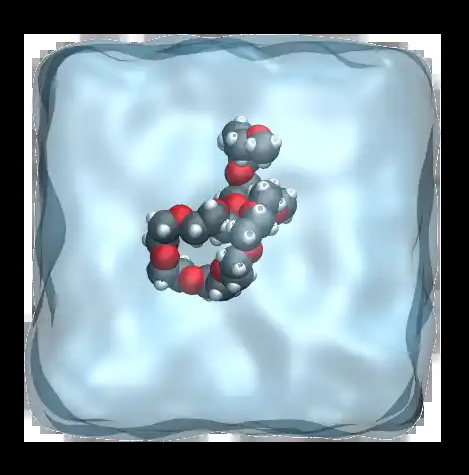
\includegraphics[width=4cm]{tutorials/level2/polymer-in-water/video-PEG-light.png}
\end{wrapfigure}

\noindent The goal of this tutorial is to use LAMMPS and
create a small hydrophilic polymer (PEG -
PolyEthylene Glycol) in a reservoir of water. 
An all-atom description is used, therefore all species considered here
are made of charged atoms connected by bonds constraints.
Once the system is created, a constant stretching force will be applied to both
ends of the polymer, and its length will be measured with time.
This tutorial was inspired by a very nice \href{https://doi.org/10.1021/acsnano.6b07071}{publication} by Liese and coworkers, in which
they compare MD simulations with force spectroscopy experiments.

\section{Bulk water}

\noindent As a first step, a rectangular box of water is created and
equilibrated at ambient temperature and ambient pressure (the PEG molecule will be added in the next sections).
Create a folder named pureH2O/. Inside this folder, create
an empty text file named input.lammps. Copy the following
lines in it:

\begin{lcverbatim}
# LAMMPS input script
units real
atom_style full
bond_style harmonic
angle_style charmm
dihedral_style charmm
pair_style lj/cut/tip4p/long 1 2 1 1 0.105 12.0
kspace_style pppm/tip4p 1.0e-4
\end{lcverbatim}

\noindent There are many differences with respect to
the previous tutorial (:ref:`lennard-jones-label`), mostly
because here a system with molecules and partial charges is
modeled (instead of neutral particles). With the unit style \textit{real},
masses are in grams per
mole, distances in Ångstroms, time in femtoseconds, energies
in Kcal/mole. With the atom style \textit{full}, each atom is a dot
with a mass and a charge. In addition, each atom can be
linked by bonds, angles, dihedrals and impropers potentials
(for example to form molecules). The \textit{bond$\_$style},
\textit{angle$\_$style}, and \textit{dihedral$\_$style} commands define the
styles of bond angle, and dihedrals used in the simulation,
respectively, and the \textit{harmonic} and \textit{charmm} keywords
impose the type of potential to use.

\begin{tcolorbox}[colback=mylightblue!5!white,colframe=mylightblue!75!black,title=About the use of charmm style]
The future merging of the water with the PEG
has already been anticipated as the \textit{charmm angle$\_$style}
and \textit{dihedral$\_$style} are requirements of the PEG's model.
A rigid water model will be used here, so the bond
and angle styles that are chosen have no consequence on the water model, they will
only matter to the PEG when it is added.
\end{tcolorbox}

\noindent With the \textit{pair$\_$style} named \textit{lj/cut/tip4p/long}, atoms
interact through both a Lennard-Jones (LJ) potential and
through Coulombic interactions. This pair style is specific to
four points water models, and automatically accounts for the
additional massless site. The six numbers are, respectively,
\begin{itemize}
\item  \textit{}1 -\textit{} the atom type for the oxygen O of the tip4p water,
\item  \textit{}2 -\textit{} the atom type for the hydrogen H of the tip4p water,
\item  \textit{}3 -\textit{} the OH bond type,
\item  \textit{}4 -\textit{} the HOH angle type,
\item  \textit{}5 -\textit{} the distance from O atom to the massless charge (here 0.105 Ångstroms is set by the TIP4P/epsilon water model),
\item  \textit{}6 -\textit{} the cutoff (here of 12 Ångstroms).
\end{itemize}

\begin{tcolorbox}[colback=mylightblue!5!white,colframe=mylightblue!75!black,title=About cutoff in molecular dynamics]
The cutoff of 12 Ångstroms applies to both LJ and Coulombic
interactions, but in a different way. For LJ \textit{cut}
interactions, atoms interact with each others only if they
are separated by a distance smaller than the cutoff. For
Coulombic \textit{long}, interaction between atoms closer than
the cutoff are computed directly, and interaction between
atoms outside that cutoff are computed in the reciprocal
space.
\end{tcolorbox}

\noindent Finally the kspace command defines the long-range solver for the (long)
Coulombic interactions. The pppm style refers to
particle-particle particle-mesh.

\begin{tcolorbox}[colback=mylightblue!5!white,colframe=mylightblue!75!black,title=Background Information (optional) -- About PPPM]
The PPPM
method is based on separating the total interaction
between particles into the sum of short-range
interactions, which are computed by direct
particle-particle summation, and long-range interactions,
which are calculated by solving Poisson's equation using
periodic boundary conditions (PBCs). 
\href{https://doi.org/10.1021/jp9518623}{Luty and van Gunsteren}
\end{tcolorbox}

\noindent Then, let us create a 3D simulation box of dimensions $8 x 3 x 3 \text{nm}^3$,
and make space for 7 atom types (1 and 2 for
the water oxygen and hydrogen, respectively, and 3, 4, 5, 6
and 7 for the PEG molecule (see below)), 6 bond types, 9
angle types, and 14 dihedrals types.

\begin{lcverbatim}
region box block -40 40 -15 15 -15 15
create_box 7 box &
bond/types 6 &
angle/types 9 &
dihedral/types 14 &
extra/bond/per/atom 2 &
extra/angle/per/atom 1 &
extra/special/per/atom 2
\end{lcverbatim}

\noindent \begin{tcolorbox}[colback=mylightblue!5!white,colframe=mylightblue!75!black,title=About extra per atom commands]
The \textit{extra/something/per/atom} commands are here for
memory allocation, they ensure that enough space is left for a
certain number of attribute for each atom. We wont worry
about those commands in this tutorial, just keep that in mind if one day you see the following
error message:
\begin{lcverbatim}
ERROR: Molecule topology/atom exceeds system topology/atom (src/molecule.cpp:1767)
\end{lcverbatim}

\noindent \end{tcolorbox}

Let us include a parameter file containing all the
parameters (masses, interaction energies, bond equilibrium
distances, etc):

\begin{lcverbatim}
include ../PARM.lammps
\end{lcverbatim}

\noindent Next to the \textit{pureH2O/} folder, create a blank file called
\textit{PARM.lammps} and copy the following lines in it:

\begin{lcverbatim}
# Mass
mass 1 15.9994 # H2O O
mass 2 1.008 # H2O H
mass 3 12.011 # CC32A
mass 4 15.9994 # OC30A
mass 5 1.008 # HCA2
mass 6 15.9994 # OC311
mass 7 1.008 # HCP1
# Pair Coeff
pair_coeff 1 1 0.18479 3.165 # H2O - TIP4P - epsilon water model
pair_coeff 2 2 0.0 0.0 # H2O H
pair_coeff 3 3 0.056 3.58141 # CC32A
pair_coeff 4 4 0.100 2.93997 # OC30A
pair_coeff 5 5 0.035 2.38761 # HCA2
pair_coeff 6 6 0.192 3.14487 # OC311
pair_coeff 7 7 0.046 0.40001 # HCP1
# Bond coeff
bond_coeff 1 0 0.9572 # H2O O-H
bond_coeff 2 222.35 1.5300
bond_coeff 3 308.79 1.1111
bond_coeff 4 359.76 1.1415
bond_coeff 5 427.715 1.1420
bond_coeff 6 544.635 0.9600
# Angle coeff
angle_coeff 1 0 104.52 0 0 # H2O H-O-H
angle_coeff 2 50.0000 109.0000 0.0000 0.0000
angle_coeff 3 26.5000 110.1000 22.5300 2.179   
angle_coeff 4 45.0000 111.5000 0.0000 0.0000 
angle_coeff 5 13.0258 109.4000 0.0000 0.0000
angle_coeff 6 35.5000 109.0000 5.4000 1.802
angle_coeff 7 55.0000 108.8900 0.0000 0.0000
angle_coeff 8 75.7000 110.1000 0.0000 0.0000
angle_coeff 9 95.0000 109.7000 0.0000 0.0000
# Dihedral coeff
dihedral_coeff 1 0.57 1 0 0
dihedral_coeff 2 0.29 2 0 0
dihedral_coeff 3 0.43 3 0 0
dihedral_coeff 4 0.59 1 180 0
dihedral_coeff 5 1.16 2 0 0 
dihedral_coeff 6 0.12 1 0 0 
dihedral_coeff 7 0.42 2 0 0
dihedral_coeff 8 0.29 3 0 0
dihedral_coeff 9 2.87 1 180 0
dihedral_coeff 10 0.03 2 0 0
dihedral_coeff 11 0.23 3 0 0
dihedral_coeff 12 1.36 1 180 0
dihedral_coeff 13 0.16 2 0 0
dihedral_coeff 14 1.01 3 0 0
\end{lcverbatim}

\noindent If you want to know which column refers to which
parameter, you can refer to the LAMMPS documentation. For
this tutorial, we will just trust that these parameters
are correct and will lead to physically consistent
behavior. Now, let us create water molecules. To do so, let us
define a water molecule using a molecule template called
\textit{H2OTip4p.txt}, and randomly create 700 of those.

\begin{lcverbatim}
molecule h2omol H2OTip4p.txt
create_atoms 0 random 700 456415 NULL mol h2omol 454756
\end{lcverbatim}

\noindent The molecule template named \textit{H2OTip4p.txt} must be \href{../../../../../inputs/level2/polymer-in-water/pureH2O/H2OTip4p.txt}{downloaded}
and saved in the same folder (named \textit{pureH2O/}) as the
input.lammps file. This template contains all the necessary structural
information of a water molecule, such as the number of atoms, 
which pair of atoms are connected by bonds, which
groups of atoms are connected by angles, etc.
Then, let us group the atoms of the water in a group named
H2O, and then delete the overlapping molecules:

\begin{lcverbatim}
group H2O type 1 2
delete_atoms overlap 2 H2O H2O mol yes
\end{lcverbatim}

\noindent Deleting overlapping molecules is required here
because the molecules where placed randomly in space by
the \textit{create$\_$atoms} command, and some of them may be too
close from each other, which may force the simulation to
crash.
The \textit{mol yes} option ensures that entire water molecules are deleted and not just single atoms.
Let us use the shake algorithm in order to constrain the
shape of the water molecules at all time. Let us also use the fix NPT to
control both the temperature and the pressure:

\begin{lcverbatim}
fix myshk H2O shake 1.0e-5 200 0 b 1 a 1 mol h2omol
fix mynpt all npt temp 300 300 100 iso 1 1 1000
\end{lcverbatim}

\noindent The parameters of the fix shake specify to
which group (H2O) the shake algorithm applied, with what
tolerance (1e-5). Still in the shake command, we also supply
the molecule template (h2omol) previously defined, and
specify to which bond/angle type shake mush apply, i.e. the
bond of type 1 and the angle of type 1.
The fix NPT allows us to impose both a temperature of 300 K (with a damping constant of 100 fs),
and a pressure of 1 atmosphere (with a damping constant of 1000 fs). With the iso keyword, the
three dimensions of the box will be re-scaled simultaneously, until the average pressure in the system 
corresponds to the desired imposed value of 1 atm.

\begin{tcolorbox}[colback=mylightblue!5!white,colframe=mylightblue!75!black,title=About rigid water model]
With shake, water molecules behave as rigid. If
you want to study the vibration of the \textit{O-H} bonds and
\textit{H-O-H} angles, you will have to use a flexible water
model. If you want to study the hydrogen transfer, you
will have to use a reactive force field,
as done in :ref:`reactive-silicon-dioxide-label`.
\end{tcolorbox}

\noindent Here only the water molecules will be rigid, the
PEG molecule (which will be added in the next part) will
be fully flexible.
Let us print the atom positions in a dump file every 1000
timesteps (i.e. 1 ps), print the temperature volume, and
density every 100 timesteps in 3 separate data files, and
print the information in the terminal every 1000 timesteps:

\begin{lcverbatim}
dump mydmp all atom 1000 dump.lammpstrj
variable mytemp equal temp
variable myvol equal vol
fix myat1 all ave/time 10 10 100 v_mytemp file temperature.dat
fix myat2 all ave/time 10 10 100 v_myvol file volume.dat
variable myoxy equal count(H2O)/3 # divide by 3 to get the number of molecule, not atom
variable mydensity equal ${myoxy}/v_myvol
fix myat3 all ave/time 10 10 100 v_mydensity file density.dat
thermo 1000
\end{lcverbatim}

\noindent \begin{tcolorbox}[colback=mylightblue!5!white,colframe=mylightblue!75!black,title=On calling variables]
Both $\$ \text{var}$ and $v_\text{var}$ can be used to call a previously defined variable named \textit{var}. 
However,  $\$ \text{var}$ returns the initial value of \textit{var}, while $v_\text{var}$ returns the instantaneous 
value of \textit{var}. 
\end{tcolorbox}

\noindent In the formula for the density (number of
molecule divided by volume), the underscore \textit{$\_$} is used to
call myvol because the volume is expected
to evolve in time when using fix NPT, but the dollar sign $\$$ is used to call myoxy as the
number of molecules is not expected to evolve during the
simulation. Note that the number of molecule changes after the
\textit{delete$\_$atoms} command is used, but this is done only before the
simulation starts.
Finally, let us set the timestep to 2.0 fs, and run the simulation for 50 ps:

\begin{lcverbatim}
timestep 2.0
run 25000
write_data H2O.data
\end{lcverbatim}

\noindent Looking at the log file, one can see how many atoms have
been deleted (the number will vary depending on the random
number you choose).

\begin{lcverbatim}
Deleted 714 atoms, new total = 1386
Deleted 476 bonds, new total = 924
Deleted 238 angles, new total = 462
\end{lcverbatim}

\noindent About 30 % the molecules were deleted due to overlapping,
together with their respective bonds and angles.
At the end of the simulation, the final state is printed
in the H2O.data file, which will be used later.

\begin{tcolorbox}[colback=mylightblue!5!white,colframe=mylightblue!75!black,title=Running LAMMPS in parallel]
This simulation may be a bit slow to complete on 1 single core.
You can speed it up by running LAMMPS on 2, 4 or even more cores, by typing:
\begin{lcverbatim}
mpirun -np 4 lmp -in input.lammps
\end{lcverbatim}

\noindent Here 4 core are used. The command may vary, depending
on your OS and LAMMPS installation.
\end{tcolorbox}

\noindent \begin{tcolorbox}[colback=mylightblue!5!white,colframe=mylightblue!75!black,title=Choosing the right number of cores]
When running a simulation in parallel using more than one CPU core, LAMMPS divides the system into
blocks, and each core is assigned to a given block. Here, as can be seen
from the terminal, when using \textit{mpirun -np 4}, LAMMPS divides 
the system into 4 blocks along the x axis:
\begin{lcverbatim}
\end{lcverbatim}

\noindent You can force LAMMPS to divide the system differently, let us say along both y and z axis,
by using the command 
\begin{lcverbatim}
processors 1 2 2
\end{lcverbatim}

\noindent However, communication between the different cores slows down the computation, so ideally you want 
to minimize the size of the surface between domains. Here the default choice of LAMMPS (i.e. processors 4 1 1)
is certainly a better choice.
If you don't know what is the best number of processors or the best way to cut the system, just perform 
a short simulation and look at the log file. For instance, if I run the simulation on 1 core I get : 
\begin{lcverbatim}
Performance: 31.567 ns/day, 0.760 hours/ns, 182.680 timesteps/s
\end{lcverbatim}

\noindent On 4 cores (keeping the default processors 4 1 1):
\begin{lcverbatim}
Performance: 109.631 ns/day, 0.219 hours/ns, 634.440 timesteps/s
\end{lcverbatim}

\noindent This is much faster, but this is not 4 times faster, because of the cost of communicating between processors.
On 4 cores and enforcing the stupid choice: processors 1 2 2, I get
\begin{lcverbatim}
Performance: 99.864 ns/day, 0.240 hours/ns, 577.919 timesteps/s
\end{lcverbatim}

\noindent Its not so bad but still not at good as 4 1 1. 
On 8 cores (the max I got), I get :
\begin{lcverbatim}
4 by 1 by 2 MPI processor grid
...
Performance: 152.106 ns/day, 0.158 hours/ns, 880.243 timesteps/s
\end{lcverbatim}

\noindent So LAMMPS chooses to divide the system once along z, and 4 times along x, and the speed is improved, but again the improvement 
is not linear with the number of cores. 
Choose carefully the best number of cores for your simulation so that you don't waste computational resource.\textit{}
Sometimes it is better to run 2 simulations on 2 cores each than 1 simulation on 4 cores.\textit{}
\end{tcolorbox}

\noindent Note that no energy minimization was performed here (NPT
molecular dynamics was started straight away). This is a
bit risky, but it works here because overlapping
molecules were deleted, and because the initial density
is very low.
If you open the dump.lammpstrj file using VMD, you should
see the system reaching its equilibrium volume:

\begin{figure}
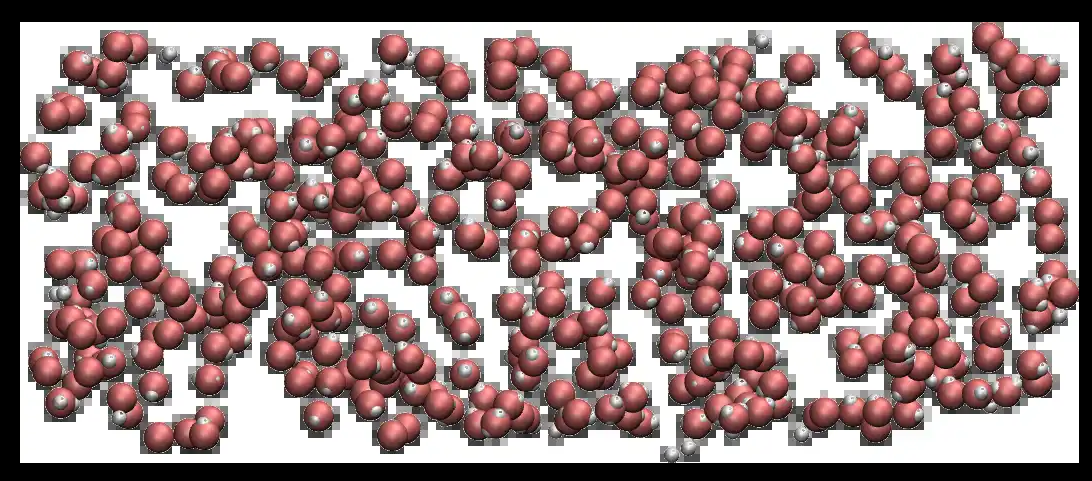
\includegraphics[width=\linewidth]{tutorials/level2/polymer-in-water/water_light.png}
\end{figure}

You can also open the temperature.dat and density.dat files
to ensure that the system converged toward an equilibrated
liquid system during the 50 ps of simulation:

\begin{figure}
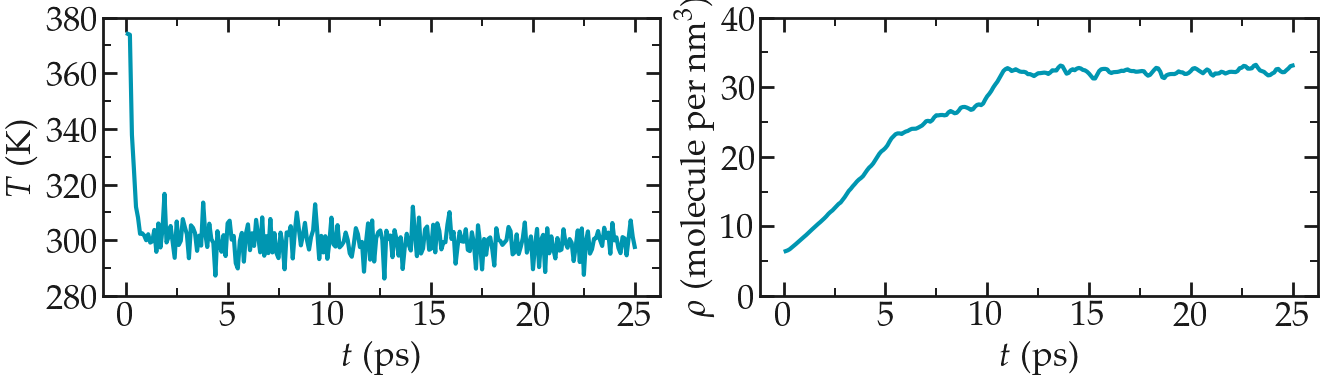
\includegraphics[width=\linewidth]{tutorials/level2/polymer-in-water/equilibration_H2O_light.png}
\end{figure}

Alternatively, you can \href{../../../../../inputs/level2/polymer-in-water/pureH2O/H2O.data}{download}
the water reservoir I have equilibrated and continue with
the tutorial.

\section{PEG molecule}

\noindent Now that the water box is ready, let us prepare the PEG
molecule in an empty box. Create a second folder next to pureH2O/, call it
singlePEG/, and create a new blank file called input.lammps
in it. Copy the same first lines as previously:

\begin{lcverbatim}
units real
atom_style full
bond_style harmonic
angle_style charmm
dihedral_style charmm
pair_style lj/cut/tip4p/long 1 2 1 1 0.105 12.0
kspace_style pppm/tip4p 1.0e-4
\end{lcverbatim}

\noindent Let us also add the \textit{special$\_$bonds} command to cancel the
Lennard-Jones interactions between the closest
atoms of a same molecule:

\begin{lcverbatim}
special_bonds lj/coul 0.0 0.0 0.5
\end{lcverbatim}

\noindent \begin{tcolorbox}[colback=mylightblue!5!white,colframe=mylightblue!75!black,title=About *special bonds*]
Usually, force fields like charmm are parametrized assuming that the first neighbors within a molecule do not
interact directly. Here, since we use 0.0 0.0 0.5, the first (for example C-O) and second (for example C-O-H) neighbors don't interact
with each other through LJ and Coulomb potentials, and therefore they only interact through direct bond interactions.
For the third neighbor (for example H-C-C-H), only half of the LJ and Coulomb interaction will be added.   
\end{tcolorbox}

\noindent Let us read the original positions for the atoms of the PEG molecule, as
well as the same parameter file as previously:

\begin{lcverbatim}
read_data init.data
include ../PARM.lammps
\end{lcverbatim}

\noindent \href{../../../../../inputs/level2/polymer-in-water/singlePEG/init.data}{Download}
the init.data file and save it in the singlePEG/ folder.
It contains the initial parameters of the PEG molecules
(atoms, bonds, charges, etc.) that was prepared using \href{https://github.com/simongravelle/PEGgenerator}{PEG generator}.
To make our life simpler later, let use use the exact same
box size for the PEG as for the water (the merging will be
simpler, see below). Open the previously generate H2O.data
file, and copy the 3 lines corresponding to the box
dimensions. In my case, its:

\begin{lcverbatim}
-21.64201909795004 21.64201909795004 xlo xhi
-8.115757161731125 8.115757161731125 ylo yhi
-8.115757161731125 8.115757161731125 zlo zhi
\end{lcverbatim}

\noindent Then, replace the box dimensions in the init.data file with
these 3 lines.
Let us print the atom positions and thermodynamic
information very frequently (because we anticipate that the
energy minimization will be short):

\begin{lcverbatim}
dump mydmp all atom 10 dump.lammpstrj
thermo 1
\end{lcverbatim}

\noindent Next, let us perform a minimisation of energy. Here, this
step is required because the initial configuration of the
PEG molecule is really far from equilibrium.

\begin{lcverbatim}
minimize 1.0e-4 1.0e-6 100 1000
\end{lcverbatim}

\noindent After the minimisation, the high resolution dump command is
cancelled, and a new dump command with lower frequency is
used (see below). We also reset the time to 0 with
\textit{reset$\_$timestep} command:

\begin{lcverbatim}
undump mydmp
reset_timestep 0
\end{lcverbatim}

\noindent The PEG is then equilibrated in the NVT ensemble (fix NVE +
temperature control = NVT). No box relaxation is required as
the PEG is in vacuum:

\begin{lcverbatim}
fix mynve all nve
fix myber all temp/berendsen 300 300 100
\end{lcverbatim}

\noindent Let us print the temperature in a file:

\begin{lcverbatim}
dump mydmp all atom 1000 dump.lammpstrj
dump_modify mydmp append yes
thermo 1000
variable mytemp equal temp
fix myat1 all ave/time 10 10 100 v_mytemp file temperature.dat
\end{lcverbatim}

\noindent The \textit{dump$\_$modify} ensures that the coordinates are written 
in the existing dump.lammpstrj file. 
Finally let us run the simulation for a very short time (10 ps):

\begin{lcverbatim}
timestep 1
run 10000
write_data PEG.data
\end{lcverbatim}

\noindent If you open the dump.lammpstrj file
using VMD, you can see the PEG molecule starting from
an extremely elongated and unrealistic shape, and 
gently equilibrating until reaching a reasonable state.

\begin{figure}
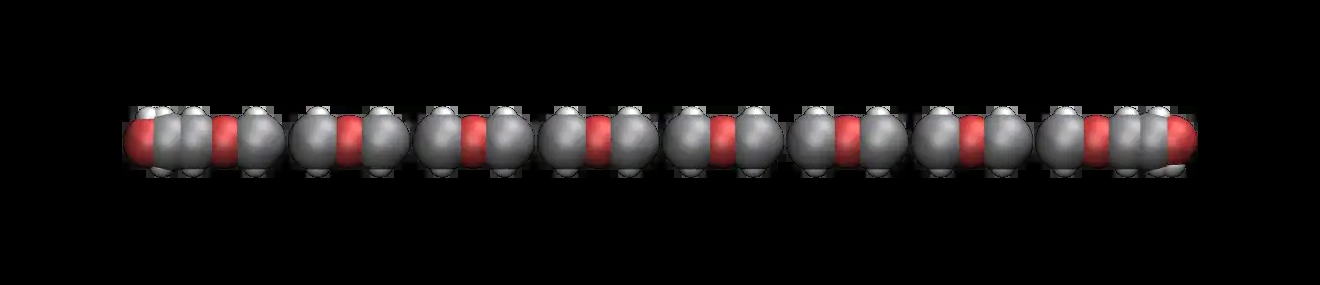
\includegraphics[width=\linewidth]{tutorials/level2/polymer-in-water/singlePEG-light.png}
\end{figure}

Alternatively, you can \href{../../../../../inputs/level2/polymer-in-water/singlePEG/PEG.data}{download}
the PEG molecule I have equilibrated and continue with the tutorial.

\section{Solvation of the PEG molecule}

\noindent Now, we merge the PEG molecule and the
water reservoir. We do it by:
\begin{itemize}
\item (1) importing both previously generated data files (PEG.data and H2O.data) into the same simulation,
\item (2) deleting the overlapping molecules, and 
\item (3) re-equilibrating the new system. 
\end{itemize}
Create a third folder alongside pureH2O/ and singlePEG/,
and call it mergePEGH2O/. Create a new blank file in it,
called input.lammps. Within input.lammps, copy the same first lines as
previously:

\begin{lcverbatim}
units real
atom_style full
bond_style harmonic
angle_style charmm
dihedral_style charmm
pair_style lj/cut/tip4p/long 1 2 1 1 0.105 12.0
kspace_style pppm/tip4p 1.0e-4
special_bonds lj/coul 0.0 0.0 0.5
\end{lcverbatim}

\noindent Then, import the two previously generated data files, as well as the same parameter file:

\begin{lcverbatim}
read_data ../singlePEG/PEG.data
read_data ../pureH2O/H2O.data add append
include ../PARM.lammps
\end{lcverbatim}

\noindent When using the \textit{read$\_$data} command more than once, one needs
to use the \textit{add append} keyword. When doing so, the
simulation box is initialized by the first \textit{read$\_$data} only, and the 
second \textit{read$\_$data} only imports additional atoms.
Let us create 2 groups to differentiate the PEG from the H2O:

\begin{lcverbatim}
group H2O type 1 2
group PEG type 3 4 5 6 7
\end{lcverbatim}

\noindent Water molecules that are overlapping with the PEG must be
deleted to avoid crashing:

\begin{lcverbatim}
delete_atoms overlap 2.0 H2O PEG mol yes
\end{lcverbatim}

\noindent Here the value of 2 Angstroms for the overlap cutoff was fixed arbitrarily,
and can be chosen through trial and error. If the cutoff is too small, the 
simulation will crash. If the cutoff it too long, too many water molecules will unnecessarily be deleted.
Finally, let us use shake to keep the water
molecules rigid, and use the NPT command to control the
temperature, as well as the pressure along the x axis:

\begin{lcverbatim}
fix myshk H2O shake 1.0e-4 200 0 b 1 a 1
fix mynpt all npt temp 300 300 100 x 1 1 1000
timestep 1.0
\end{lcverbatim}

\noindent The box dimension will only adjust along the x axis here.
Once more, let us dump the atom positions and a few
information about the evolution simulation:

\begin{lcverbatim}
dump mydmp all atom 100 dump.lammpstrj
thermo 100
variable mytemp equal temp
variable myvol equal vol
fix myat1 all ave/time 10 10 100 v_mytemp file temperature.dat
fix myat2 all ave/time 10 10 100 v_myvol file volume.dat
\end{lcverbatim}

\noindent Let us also print the total enthalpy:

\begin{lcverbatim}
variable myenthalpy equal enthalpy
fix myat3 all ave/time 10 10 100 v_myenthalpy file enthalpy.dat
\end{lcverbatim}

\noindent Finally, let us perform a short equilibration and print the
final state in a data file:

\begin{lcverbatim}
run 10000
write_data mix.data
\end{lcverbatim}

\noindent If you open the dump.lammpstrj file using VMD, you should
see that the box dimension slightly shrink along x.
The system looks like that:

\begin{figure}
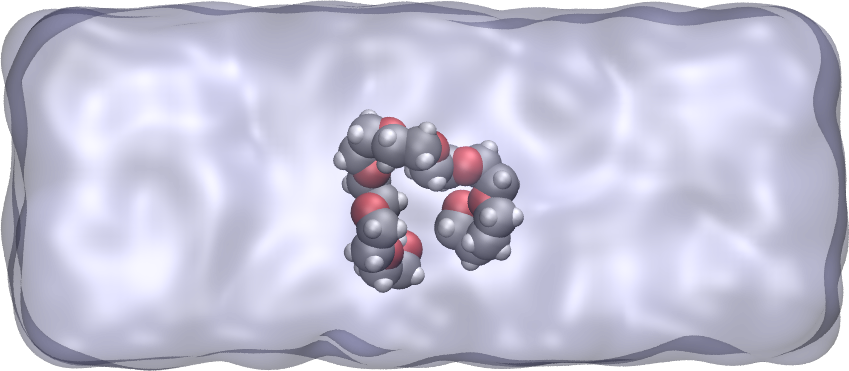
\includegraphics[width=\linewidth]{tutorials/level2/polymer-in-water/solvatedPEG_light.png}
\end{figure}

\section{Stretching the PEG molecule}

\noindent Here, a constant forcing is applied to the two ends of the
PEG molecule until it stretches. Create a new folder next
to the 3 previously created folders, call it pullonPEG/
and create a new input file in it called input.lammps.
First, let us create a variable containing the magnitude
of the force we are going to apply. The force magnitude is
chosen to be large enough to overcome the thermal
agitation and the entropic contribution from both water
and PEG molecules (it was chosen by trial and error). Copy
in the input file:

\begin{lcverbatim}
variable f0 equal 5 # kcal/mol/A # 1 kcal/mol/A = 67.2 pN
\end{lcverbatim}

\noindent Then, as previouly, copy:

\begin{lcverbatim}
units real
atom_style full
bond_style harmonic
angle_style charmm
dihedral_style charmm
pair_style lj/cut/tip4p/long 1 2 1 1 0.105 12.0
kspace_style pppm/tip4p 1.0e-4
special_bonds lj/coul 0.0 0.0 0.5
\end{lcverbatim}

\noindent Start the simulation from the equilibrated PEG + water
system, and include again the parameters:

\begin{lcverbatim}
read_data ../mergePEGH2O/mix.data
include ../PARM.lammps
\end{lcverbatim}

\noindent Then, let us create 4 atom groups: H2O and PEG (as
previously) as well as 2 groups containing one single atom
corresponding respectively to the oxygen atoms located at the
ends of the PEG molecule:

\begin{lcverbatim}
group H2O type 1 2
group PEG type 3 4 5 6 7
group oxygen_end1 id 65
group oxygen_end2 id 4
\end{lcverbatim}

\noindent Let us print again the atom positions in a dump:

\begin{lcverbatim}
dump mydmp all atom 1000 dump.lammpstrj
# write_dump all atom dump.lammpstrj
# dump myxtc xtc atom 1000 dump.xtc
\end{lcverbatim}

\noindent \begin{tcolorbox}[colback=mylightblue!5!white,colframe=mylightblue!75!black,title=Use less disk space by using the xtc format]

To generate smaller dump files, use the
compressed \textit{xtc} format. You can do it by commenting the
mydmp line and by uncommenting both the \textit{write$\_$dump} and
\textit{myxtc} lines. Note that \textit{xtc} files are compressed, and not readable
by humans, contrarily to the LAMMPS native format \textit{lammpstrj}. 
\end{tcolorbox}

\noindent Let us use a simple thermostating for all atoms 
and use shake for the rigid water molecules:

\begin{lcverbatim}
timestep 1
fix myshk H2O shake 1.0e-4 200 0 b 1 a 1
fix mynvt all nvt temp 300 300 100
\end{lcverbatim}

\noindent \begin{lcverbatim}
variable mytemp equal temp
fix myat1 all ave/time 10 10 100 v_mytemp file temperature.dat
variable x1 equal xcm(oxygen_end1,x)
variable x2 equal xcm(oxygen_end2,x)
variable delta_x equal abs(v_x1-v_x2)
fix myat2 all ave/time 10 10 100 v_delta_x file end-to-end-distance.dat
thermo 5000
\end{lcverbatim}

\noindent Finally, let us run the simulation for 10 ps (without
any external forcing):

\begin{lcverbatim}
run 10000
\end{lcverbatim}

\noindent This 10 ps serves as an extra small equilibration. In principle, 
it is not necessary as equilibration was properly performed during the 
previous step. Then, let us apply a forcing on the 2 oxygen atoms using 2
\textit{add$\_$force} commands, and run for 100 ps (for a total duration
of the simulation of 110 ps):

\begin{lcverbatim}
fix myaf1 oxygen_end1 addforce ${f0} 0 0
fix myaf2 oxygen_end2 addforce -${f0} 0 0
run 50000
\end{lcverbatim}

\noindent If you open the \textit{dump.lammpstrj} file using \textit{VMD}, you should
see this:

\begin{figure}
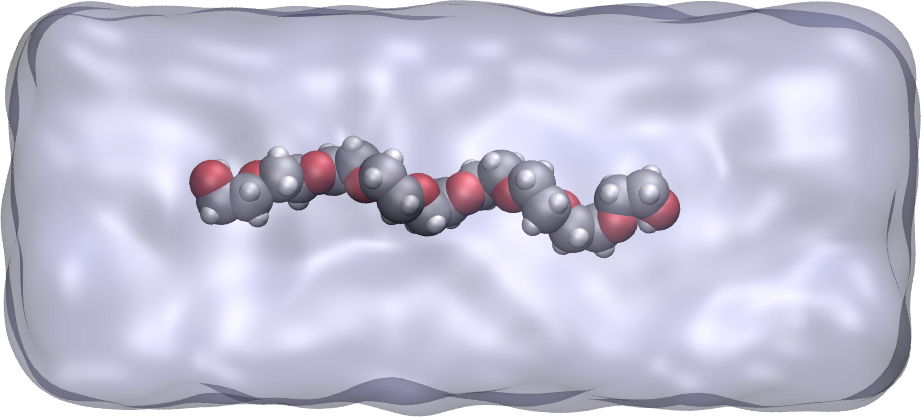
\includegraphics[width=\linewidth]{tutorials/level2/polymer-in-water/pulled_peg_light.png}
\end{figure}

The evolution of the end-to-end
distance over time shows the PEG adjusting
to the external forcing:

\begin{figure}
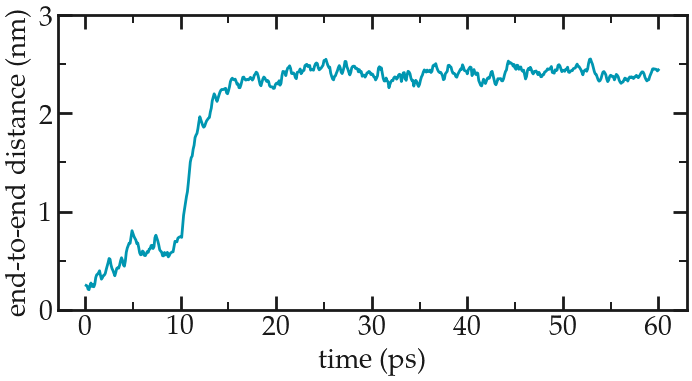
\includegraphics[width=\linewidth]{tutorials/level2/polymer-in-water/distance-light.png}
\end{figure}

\section{What now?}

\noindent Now that you have completed this relatively advanced molecular dynamics tutorials, and 
that all input scripts are working, I suggest you to mess around with the inputs and 
try to trigger warnings and error. The more warning and error you trigger from a working input, the 
easier it will be to solve future issue in your own input. 

\section{Going further with exercises}

\noindent \subsection{Generate a PEG-H2O mixture}

Use the same script and a similar procedure and create a
PEG-H2O mixture with several PEG molecules hydrated in a
cubic box.

\begin{tcolorbox}[colback=mylightblue!5!white,colframe=mylightblue!75!black,title=Hints]
LAMMPS has internal commands allowing to replicate
a molecule or a system.
There is no obligation to equilibrate the water molecules separately from the PEG,
as we did here. You can also create the water molecules directly around the PEG molcule
using the \textit{create$\_$atom} command.
\end{tcolorbox}

\noindent \subsection{End-to-end distance}

Create 2 simulations, one with a PEG molecule in vacuum, one
with a PEG molecule in water, and measure their respective
end-to-end equilibrium distance. PEG are hydrophilic and
form hbonds with water molecules, therefore, when immersed
in water, PEG molecules slightly unfold, which changes the
equilibrium end-to-end distance.

\subsection{Post-mortem analysis}

\noindent In today research, most data analyses are
done after the simulation is over, and it is important for
LAMMPS users to know how to do it.
Import the trajectory using Python, and re-extract the
end-to-end distance.

\begin{tcolorbox}[colback=mylightblue!5!white,colframe=mylightblue!75!black,title=Hints]
You can import \textit{lammpstrj} file using \textit{MDAnalysis} in \textit{Python}:
\begin{lcverbatim}
u = mda.Universe("dump.lammpstrj", format = "LAMMPSDUMP")
\end{lcverbatim}

\noindent \end{tcolorbox}

